\chapter{Contexto Geológico}

A área de estudo enquadra-se geolologicamente no Rift Continental do Sudeste do Brasil sobre terrenos policíclicos referíveis ao sul do Cinturão de Dobramentos Ribeira, como explica \cite{Riccomini_1989} em seu trabalho. Essa faixa é composta por rochas metamórficas,
migmatitos e granitóides relacionados ao Ciclo Orogenético Brasiliano, como citam \cite{kuhn_metamorphic_2004}, \cite{heilbron_evolution_2010} e \cite{valeriano_u_pb_2011}. Essa zona geológica é intulada por \cite{Almeida_Carneiro_1998} como Planalto Atlântico . Encontra-se nessa região retrabalhamento de ciclos orogênicos pretéritos e o conjunto lito1ógico está recortado por sistema de falhamentos transcorrentes (zonas de cisalhamento) orientados segundo a estruturação regional, direção ENE a EW, segundo \cite{Hasui_Sadowski_1976}.

\begin{figure}[!ht]
\centering
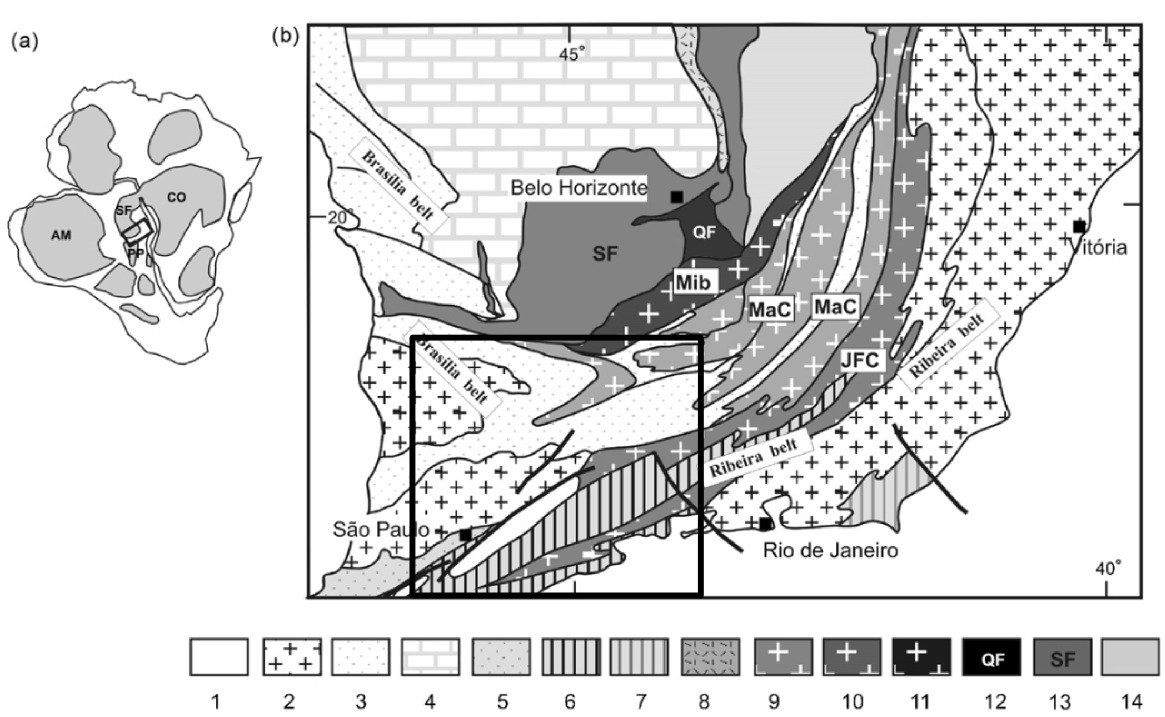
\includegraphics[scale=0.5]{mapa_geologico.png}
\caption{a-Localização da área não Período pré-Brasiliano. b-Mapa tectônico da Região do Sudeste do Brasil. Legenda: 1-Sedimentos Fanerozóicos; 2-Arcos magmáticos Neoproterozóicos fazer Brasília, cinturões Ribeira e Araçuaí; Marginais 3 Sequências passivas Neoproterozóicas; 4-Grupo Bambuí; 5-Terreno Apiaí; 6-Terreno Embú e Paraíba do Sul; 7-Terreno Cabo Frio; 8-Sequências Mesoproterozóicas do Espinhaço; 9-Cinturão Mineiro; 10-Complexo Mantiqueira e Rochas Relacionadas; 11-Complexo Juiz de Fora Misturado com Sequências Neoproterozóicas; 12-Supergrupo Minas não Quadrilátero Ferrífero; 13-Sucessões Arqueanas nenhum sul do Cráton do São Francisco; 14-Terreno Guanhães.}
\label{mapa_geologico}
\end{figure} 

